\documentclass[tikz, border=1mm]{standalone}

\begin{document}
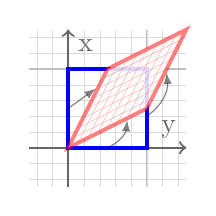
\begin{tikzpicture}

    % Draw minor grid lines (0.2 step)
    \draw[gray!30, ultra thin, step=0.2] (-.5,-.5) grid (1.5,1.5);
    
    % Draw major grid lines (1 step)
    \draw[gray!50, thin, step=1] (-.5,-.5) grid (1.5,1.5);
        
    % Draw axes
    \draw[thick,->,color=black!60] (0,-.5) -- (0,1.5) node[anchor=north west] {x};
    \draw[thick,->,color=black!60] (-.5,0) -- (1.5,0) node[anchor=south east] {y};

    % Draw unit square
    \draw[blue, line width=.5mm] (0,0) -- (1,0) -- (1,1) -- (0,1) -- cycle;
    \draw[red, line width=.5mm, opacity = .5, fill=white, fill opacity = .85] (0,0) -- (1, .5) -- (1.5,1.5) -- (.5,1) -- cycle;

    % \draw[-latex, opacity=.5] (1,1) to (1.5, 1.5); 
    \draw[-latex, opacity=.5] (.5,0) to [bend right] (.75, .35);
    \draw[-latex, opacity=.5] (0,.5) to  (.35,.75);
    \draw[-latex, opacity=.5] (1,.4) to [bend right] (1.25,.95);
    % \draw[-latex, opacity=.5] (.4,1) to [bend left] (.95,1.25);

    \foreach \x in {0.125, 0.250, 0.375, 0.500, 0.625, 0.750, 0.875} {
      \draw[red!50, ultra thin] (\x, .5 * \x) -- (.5 + \x, 1 + .5 * \x);
      \draw[red!50, ultra thin] (.5 * \x, \x) -- (1 + .5*\x, .5 + \x);
    }
\end{tikzpicture}
\end{document}
